\noindent In this tutorial, we describe steps for setting up a Maven
project that uses {\tt libSBOLj} in Eclipse, and explain how we use SBOL
2.0 to represent the function of a state-of-the-art design, namely a
CRISPR-based repression module Kiani~\textit{et
  al.}~\cite{kiani2014crispr} using the Java library. 

\section*{Set up Maven plugins in Eclipse}
In this section, we describe steps for installing Maven plugins in Eclipse. The Eclipse version used is Luna Service Release 2 (4.4.2). Here are the steps:
\begin{enumerate}
\item In Eclipse, go to Help and select Install New Software, 
\item Add a new software site: Name = slf4j, URL = \url{http://www.fuin.org/p2-repository/}, 
\item Select this site to work with, expand Maven osgi-bundles, and select slf4j.api, 
\item Click Next and follow the installation process, 
\item Add a new software site: Name = Maven Plugins, URL = \url{http://download.eclipse.org/technology/m2e/releases}, 
\item Select this site to work with, expand Maven Integration for Eclipse, and select m2e - Maven Integration for Eclipse, and
\item Click Next and follow the installation process.
\end{enumerate}

\section*{Creating a new project}
After the Maven plugin is installed, we are now ready to create a new Maven project in Eclipse. The following text describe the necessary steps. 

In the package explorer window, right click and select {\bf New $\rightarrow$ Other}.
\begin{center}
  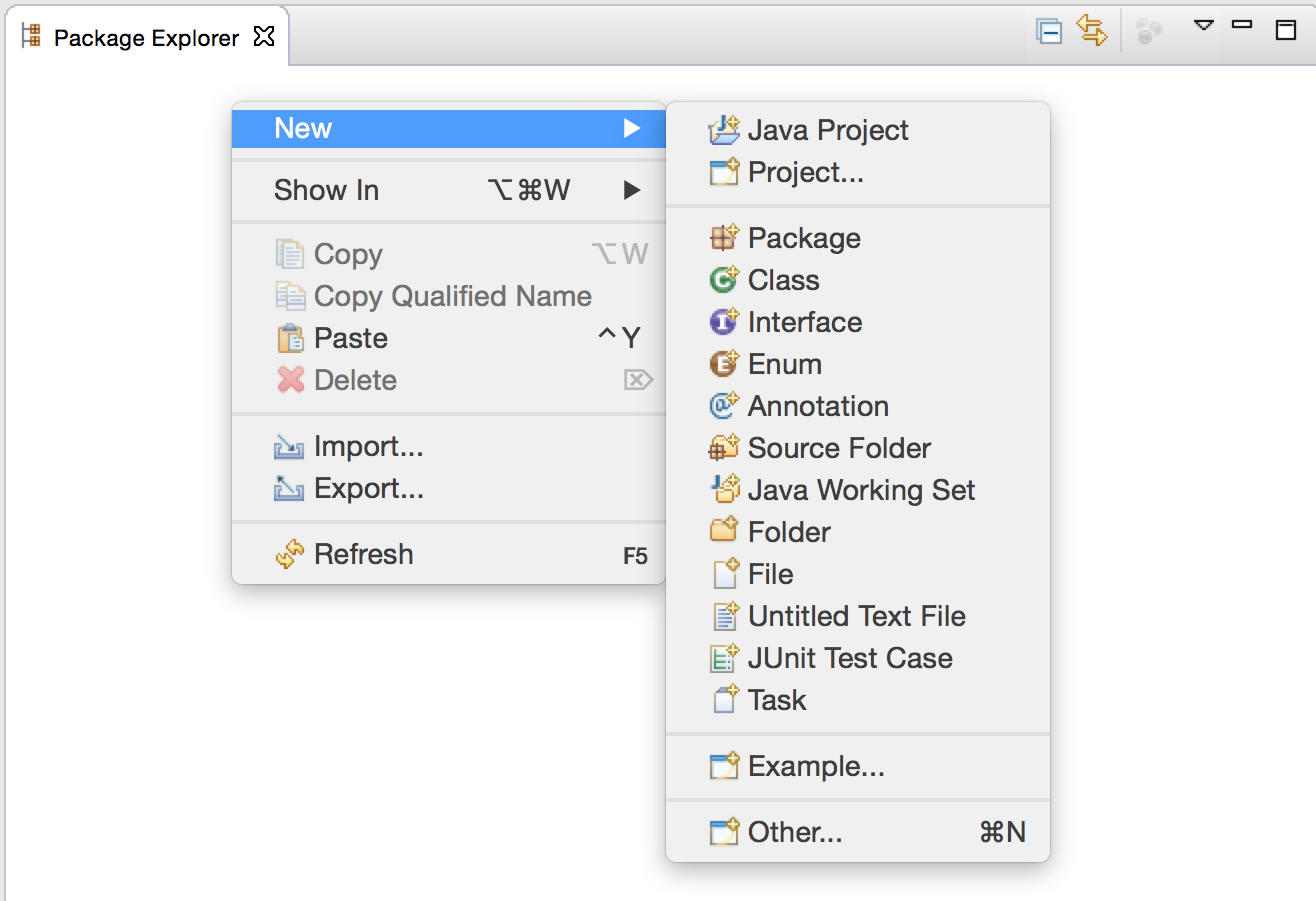
\includegraphics[width=0.8\textwidth]{figures/createNewMavenProject1}
\end{center}

Under the {\bf Maven} folder, choose {\bf Maven Project}, and then follow the default options for the project setup.
\begin{center}
  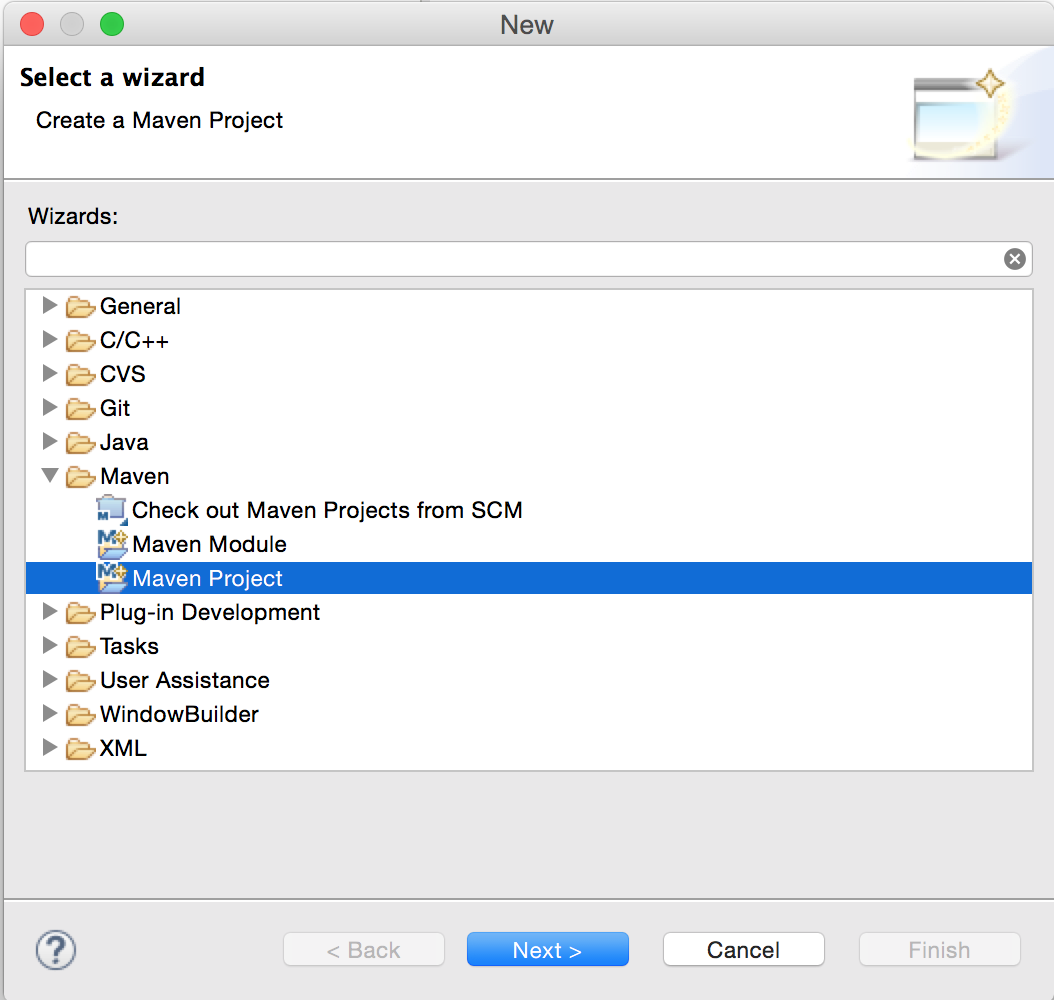
\includegraphics[width=0.75\textwidth]{figures/createNewMavenProject2}
\end{center}

% \begin{center}
%   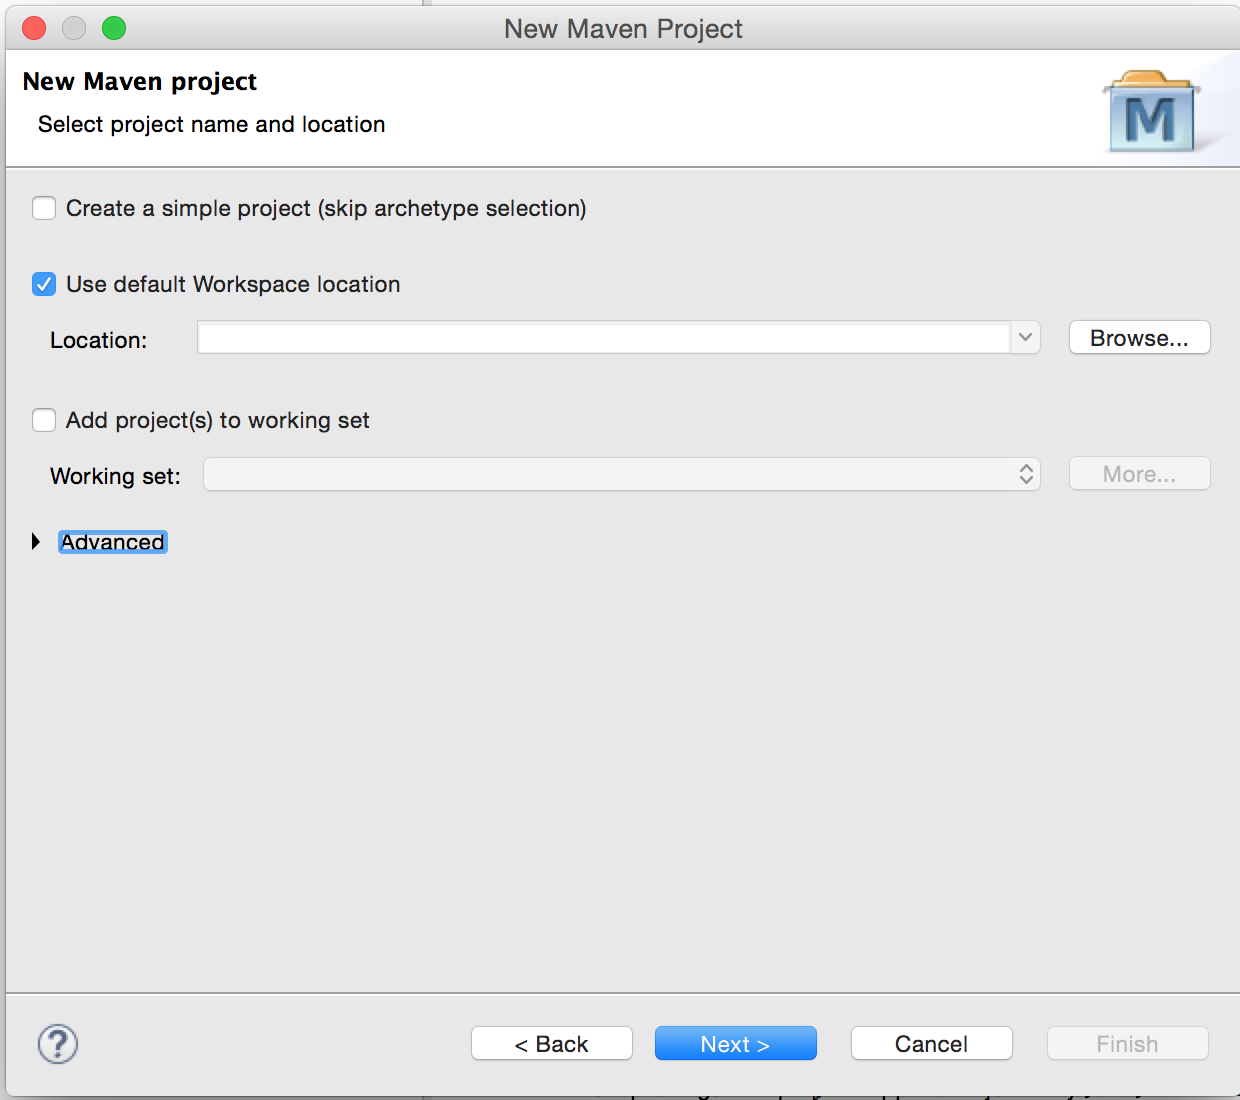
\includegraphics[width=0.8\textwidth]{figures/createNewMavenProject3}
% \end{center}

\begin{center}
  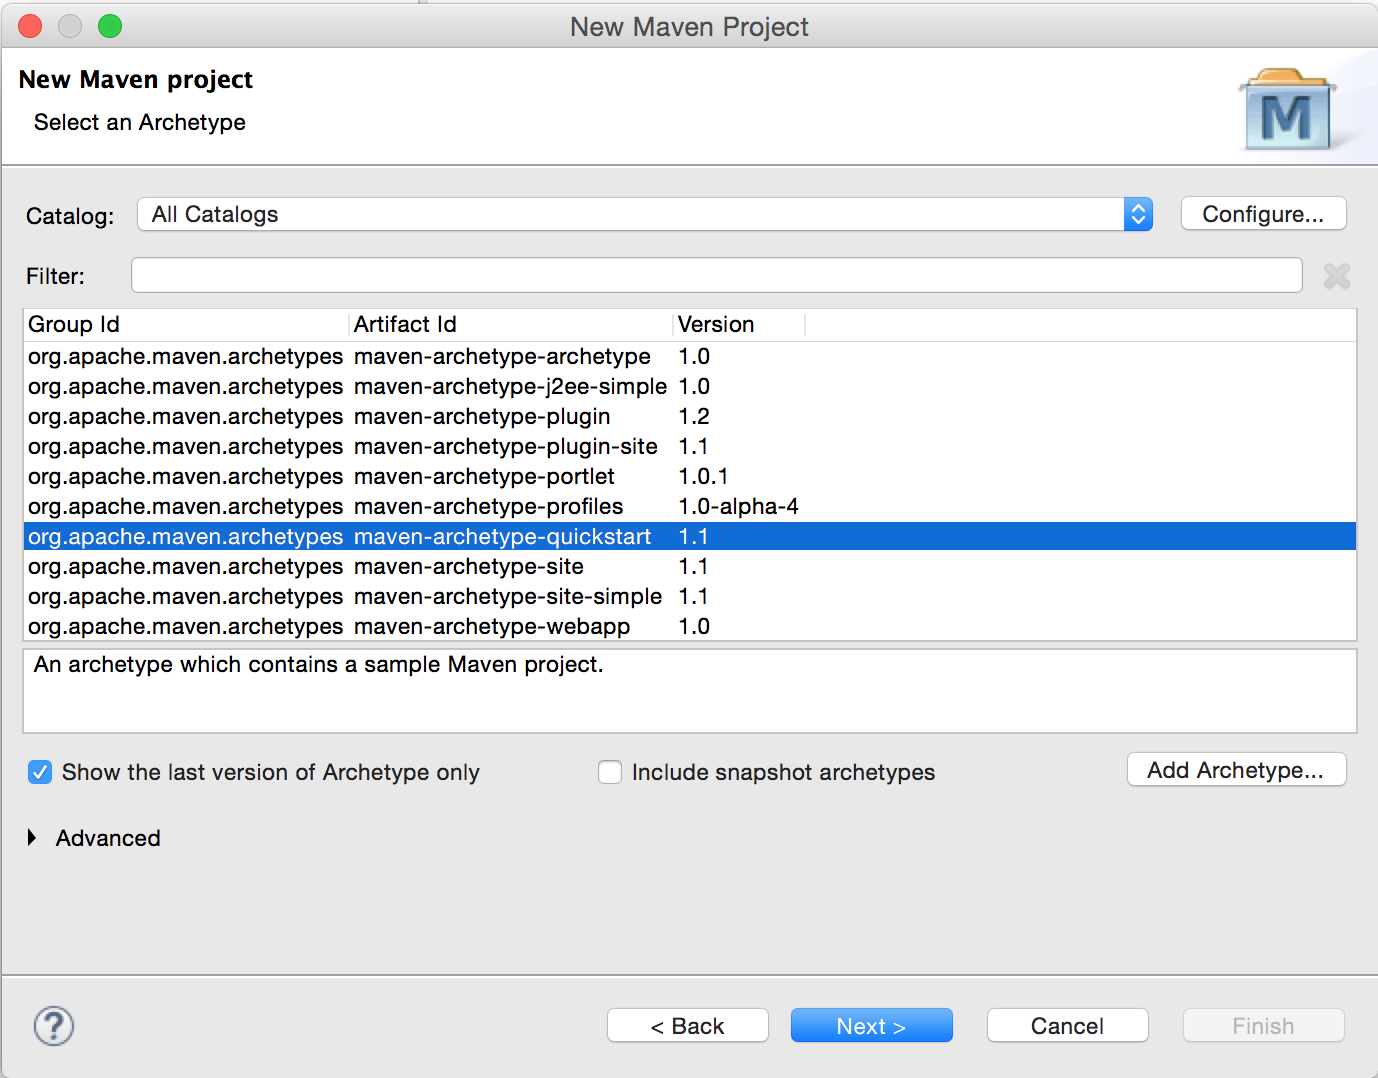
\includegraphics[width=0.75\textwidth]{figures/createNewMavenProject4}
\end{center}

In the window for specifying archetype parameters, you may type your group ID and artifact ID. In this tutorial, they are specified as shown below. 
\begin{center}
  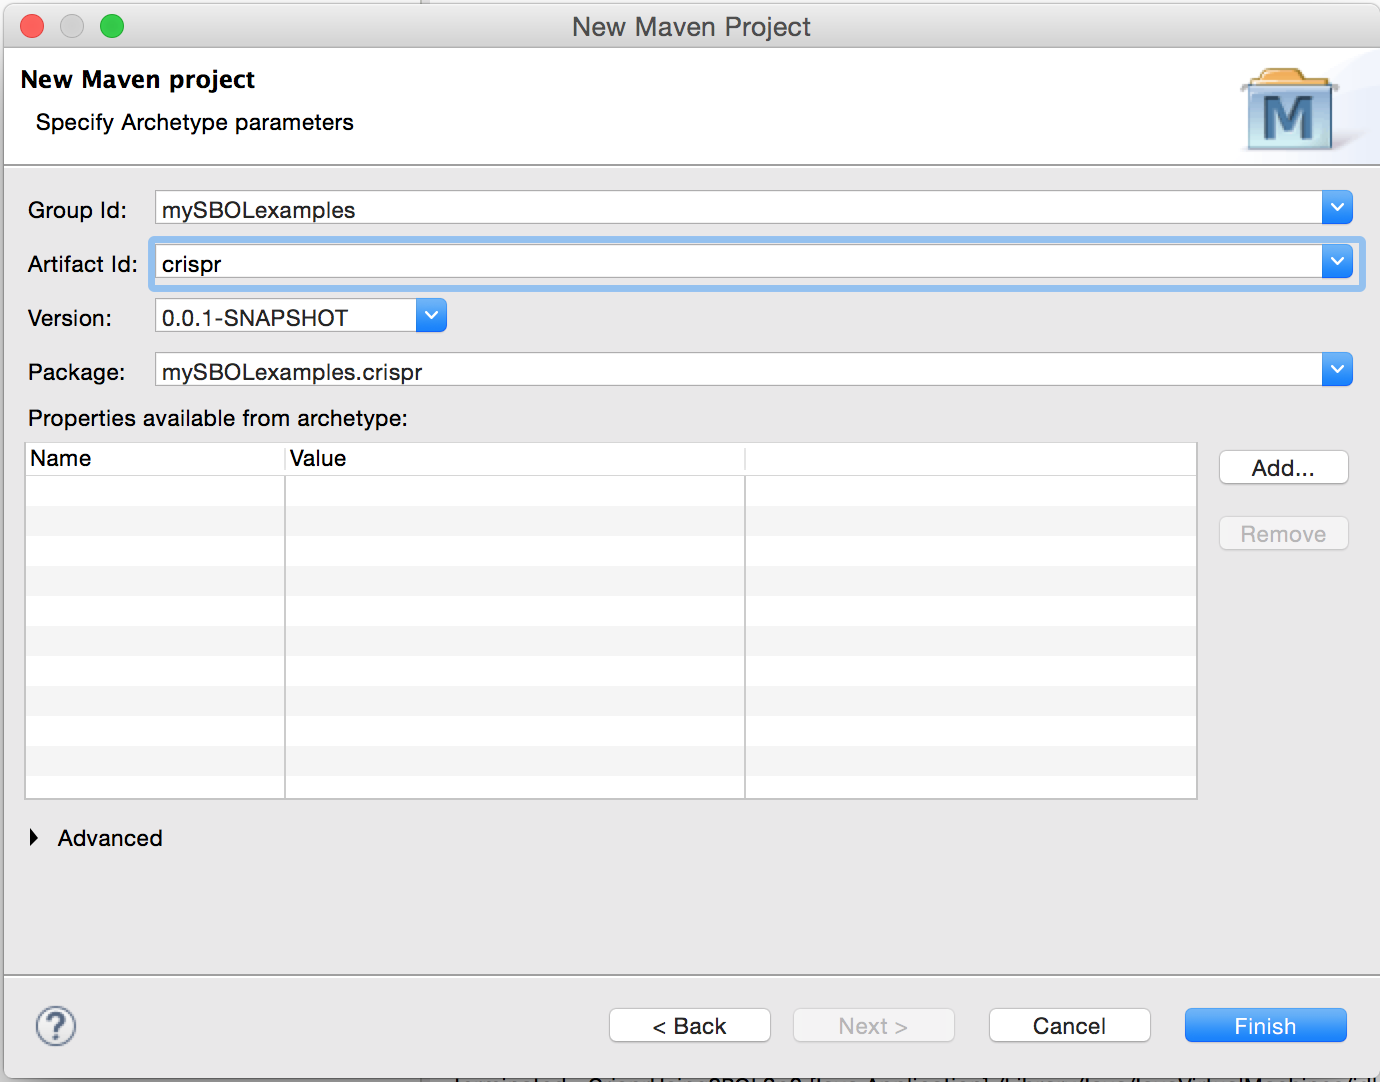
\includegraphics[width=0.8\textwidth]{figures/createNewMavenProject5}
\end{center}

Once the project setup is finished, you should be able to see two Java source folders, a {\bf JRE System Library} and a {\bf Maven Dependencies} library, and a {\bf pom.xml} file. 
\begin{center}
  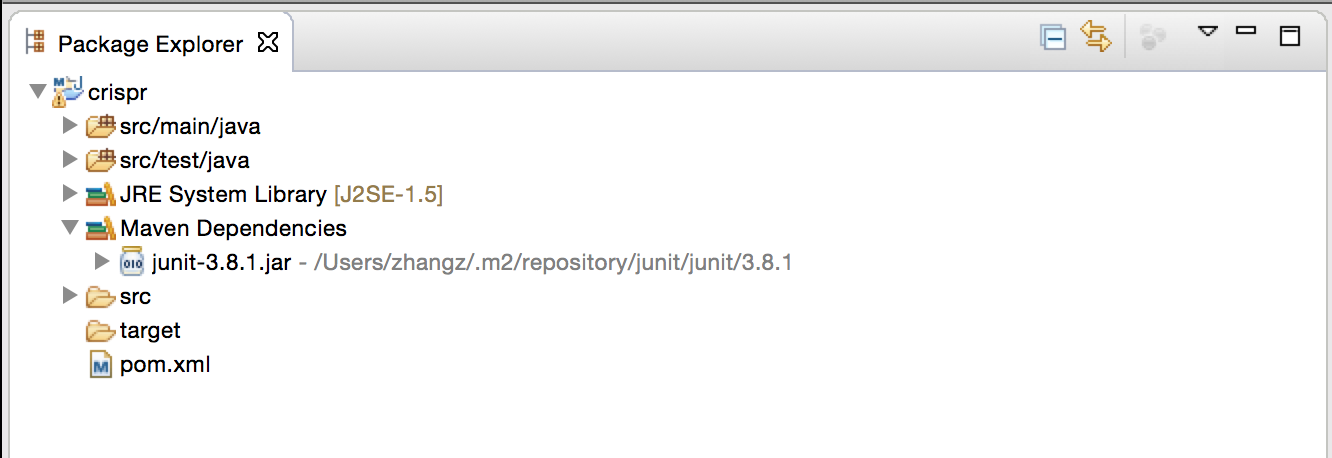
\includegraphics[width=0.8\textwidth]{figures/createNewMavenProject6}
\end{center}

It is possible that the JRE System Library created by Maven is not compatible with the installed JREs. In the screenshot shown below, it is set to {\bf J2SE-1.5}, but the Maven compiler is compatible with {\bf JavaSE-1.7} instead. To change it, right-click on JRE System Library, and select {\bf Build Path $\rightarrow$ Configure Build Path}. 
\begin{center}
  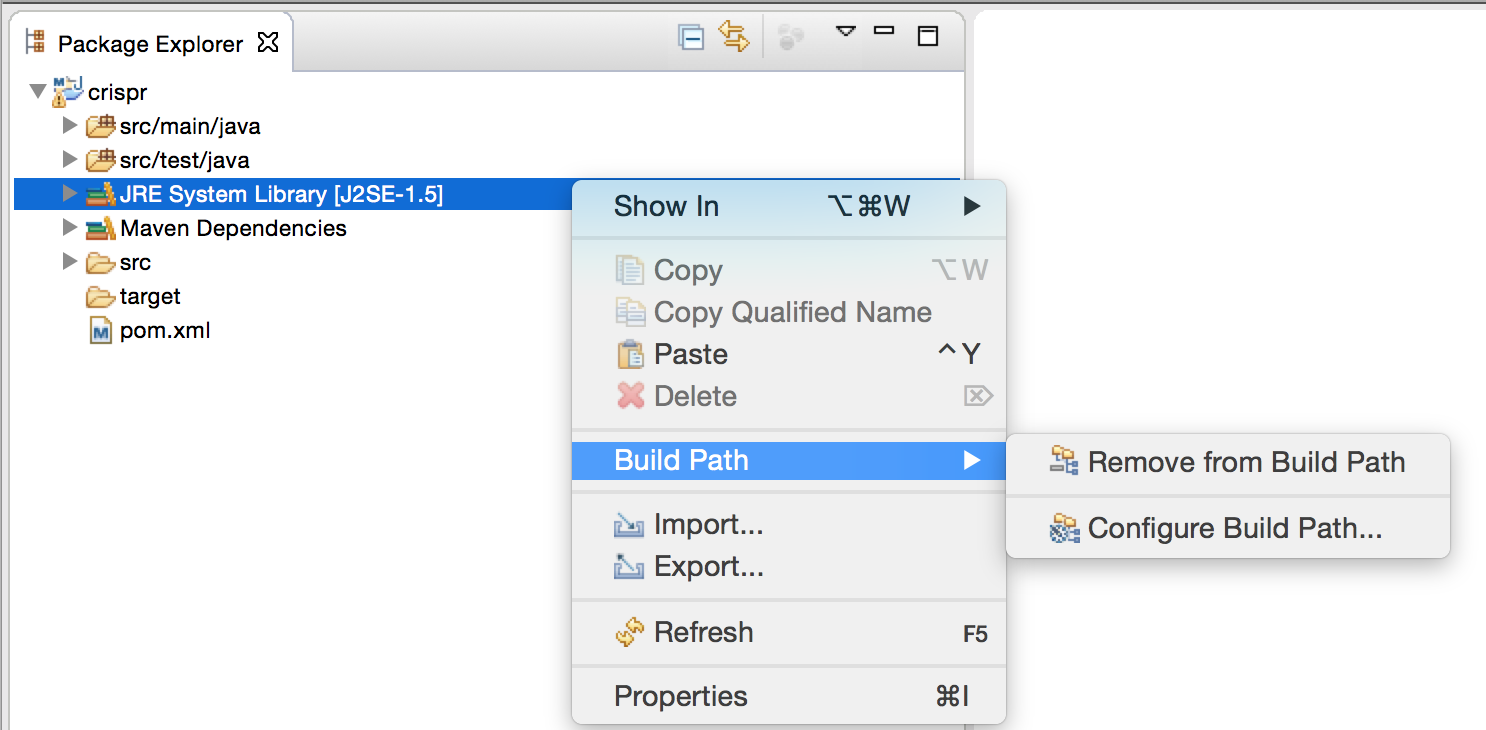
\includegraphics[width=0.8\textwidth]{figures/createNewMavenProject7}
\end{center}

In the popup properties window, select {\bf Edit} under {\bf Libraries}. 
\begin{center}
  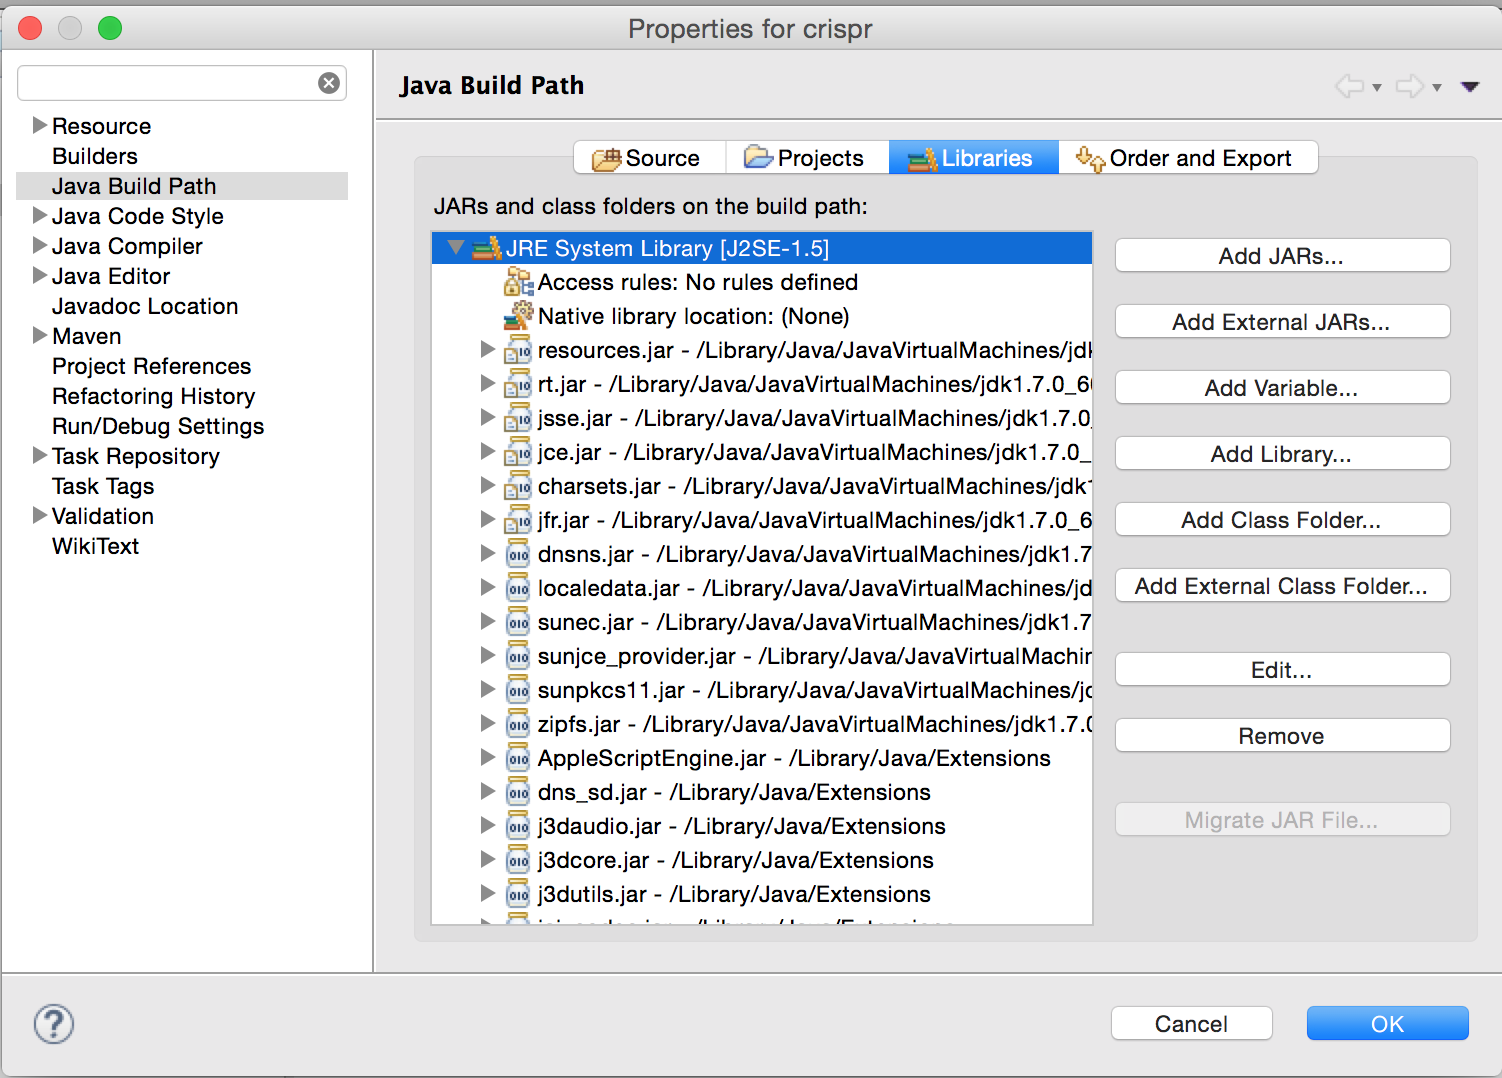
\includegraphics[width=0.8\textwidth]{figures/createNewMavenProject8}
\end{center}

We can now change the execution environment to JavaSE-1.7 as shown below. 
\begin{center}
  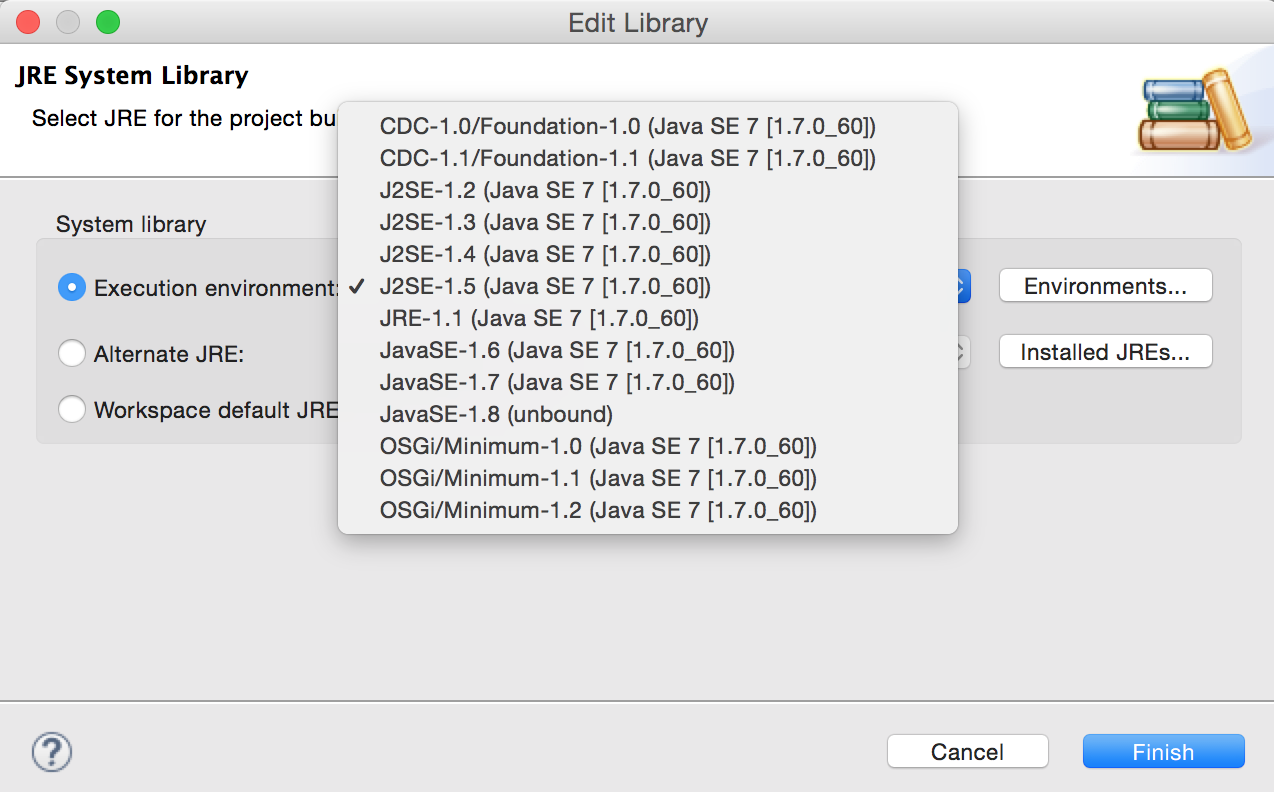
\includegraphics[width=0.8\textwidth]{figures/createNewMavenProject9}
\end{center}

This solution, however, is temporary. If we right-click on the ``crispr'' project and then select {\bf Maven $\rightarrow$  Update Project}, the JRE will reset itself back to J2SE-1.5. 
\begin{center}
  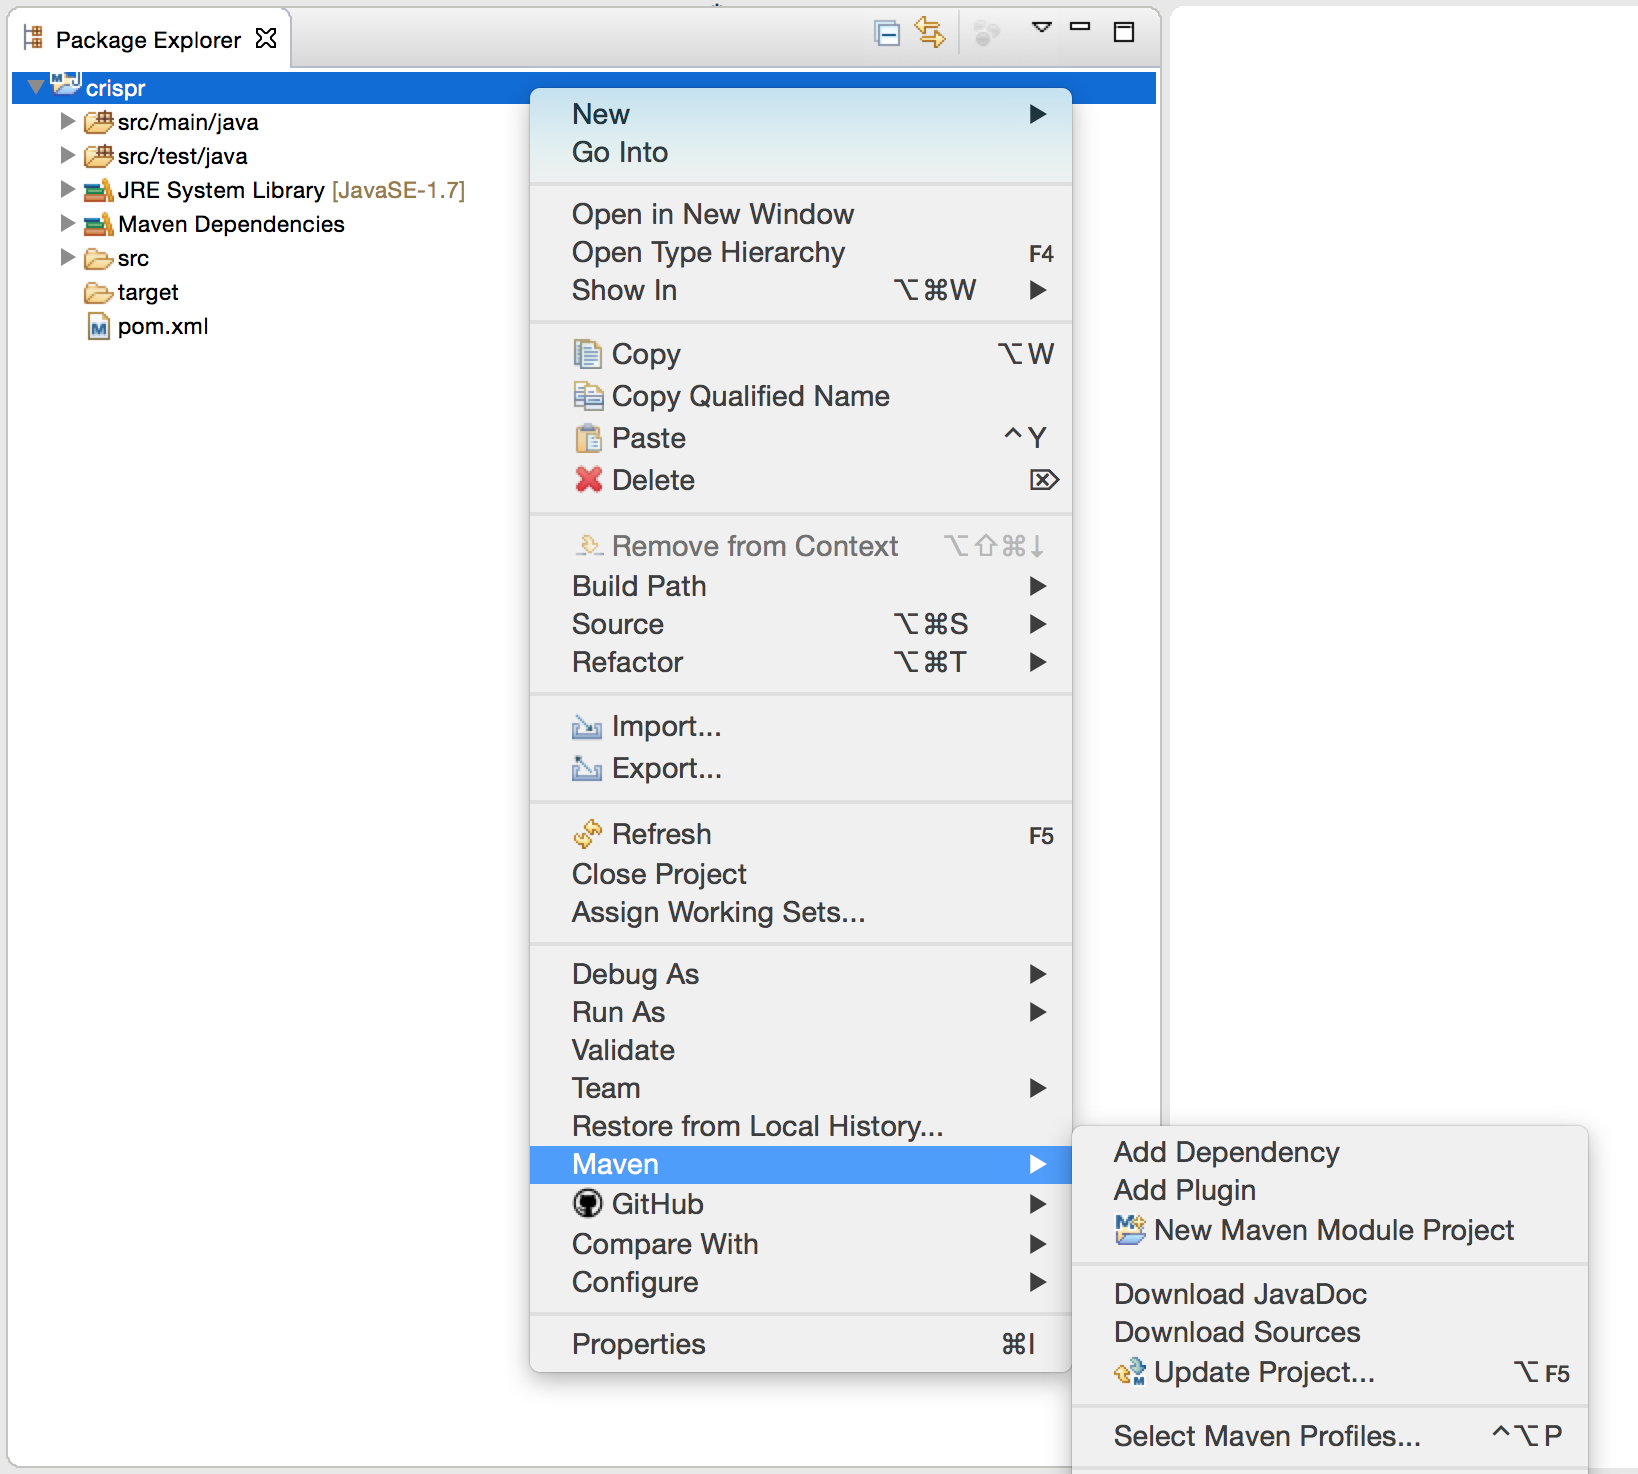
\includegraphics[width=0.8\textwidth]{figures/createNewMavenProject10}
\end{center}

A permanent fix would be to manually add the plugin management information below to the pom.xml file.

\begin{minipage}{\textwidth} 
\begin{lstlisting}[language=xml,basicstyle=\footnotesize\ttfamily]
<build>
    <pluginManagement>
        <plugins>
            <plugin>
                <groupId>org.apache.maven.plugins</groupId>
                <artifactId>maven-compiler-plugin</artifactId>
                <version>3.1</version>
                <configuration>
                    <source>1.7</source>
                    <target>1.7</target>
                </configuration>
            </plugin>
        </plugins>
    </pluginManagement>
</build>
\end{lstlisting}
\end{minipage}

The pom.xml should look like the one shown below after this modification. Remember to save the file and then do {\bf Maven $\rightarrow$  Update Project}.

\begin{minipage}{\textwidth} 
\lstinputlisting[language=xml,basicstyle=\footnotesize\ttfamily]{pom.xml}
\end{minipage}

\section*{Adding {\tt libSBOLj} as dependency}
We are now ready to add libSBOLj as a Maven dependency. This can be easily done by right-clicking on the ``crispr'' project and then select {\bf Maven $\rightarrow$ Add Dependency}.
% \begin{center}
%   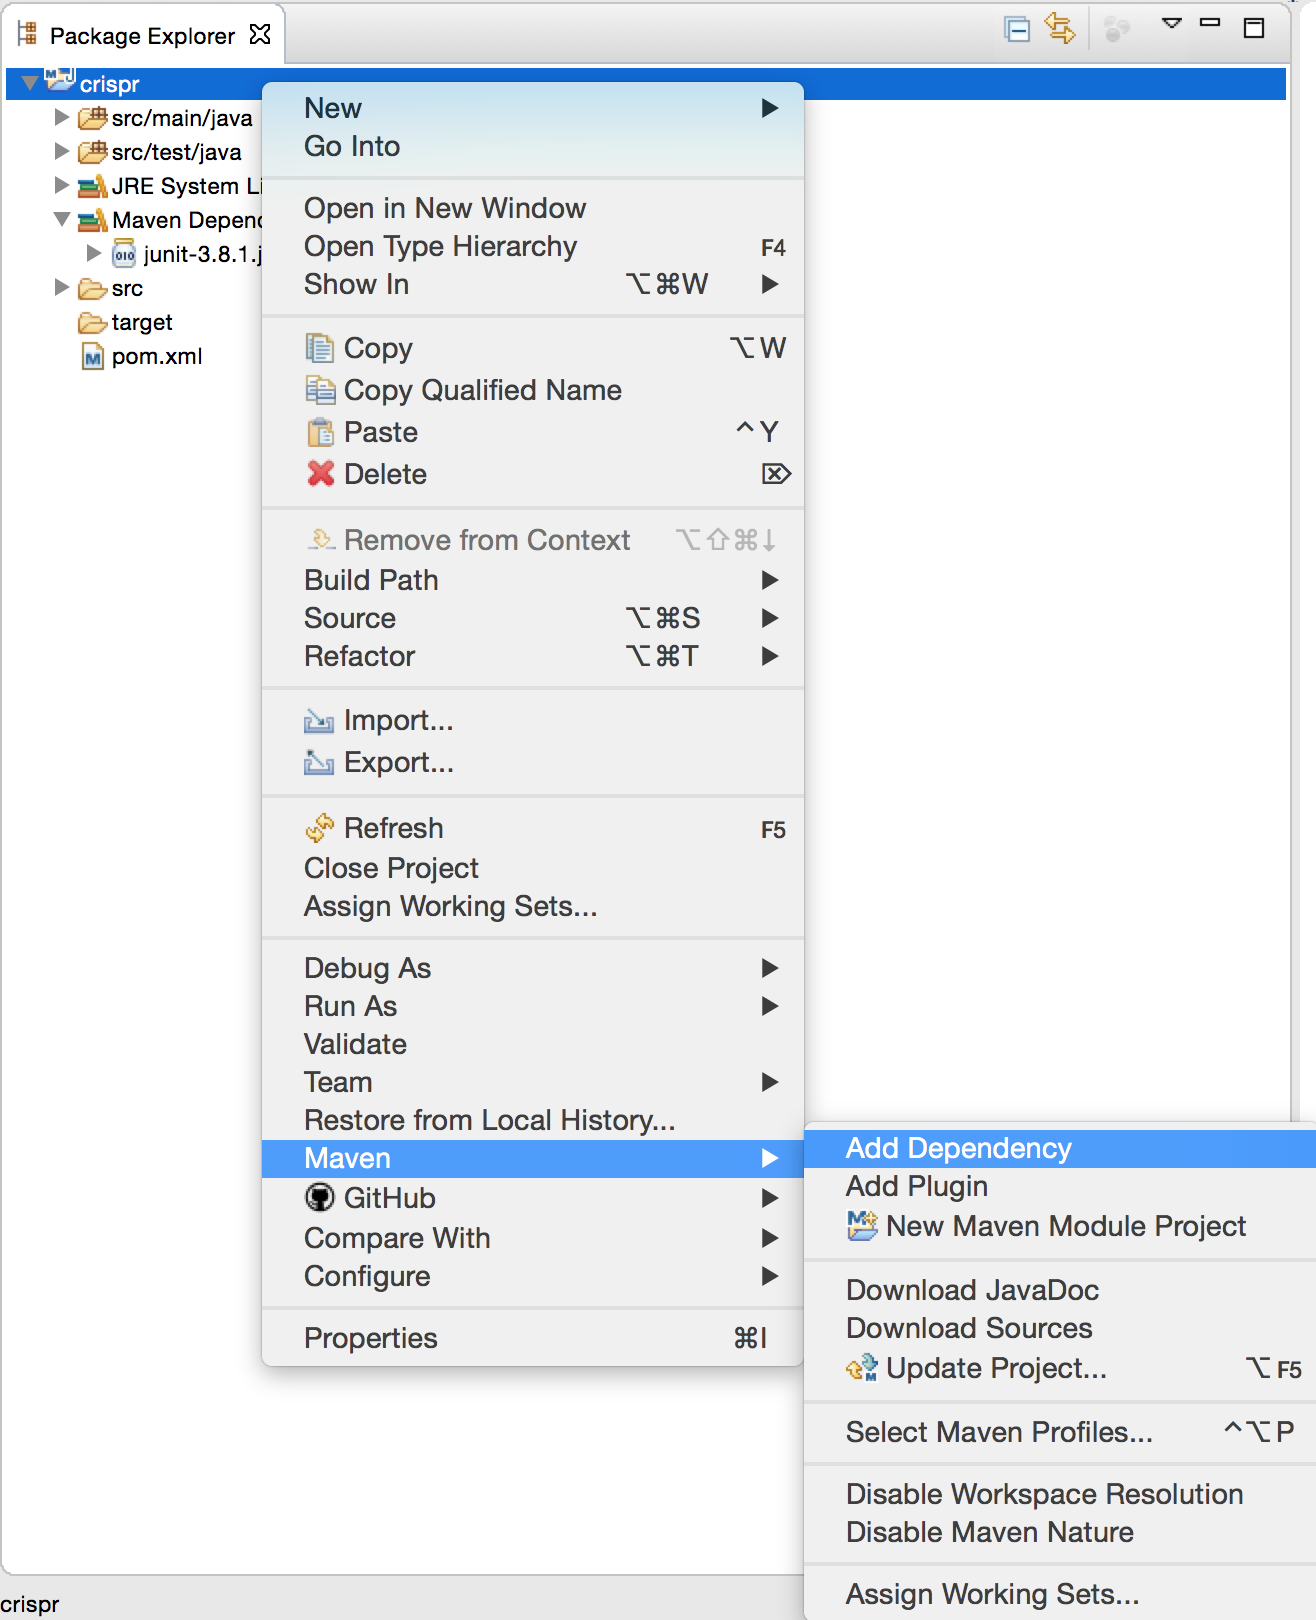
\includegraphics[width=0.55\textwidth]{figures/addMavenDependency1}
% \end{center}
In the popup window shown below, fill in the information for the {\tt libSBOLj} library. The group ID is {\bf org.sbolstandard}, and the artifact ID is {\bf libSBOLj} and the version is {\bf 2.1.0}. 
\begin{center}
  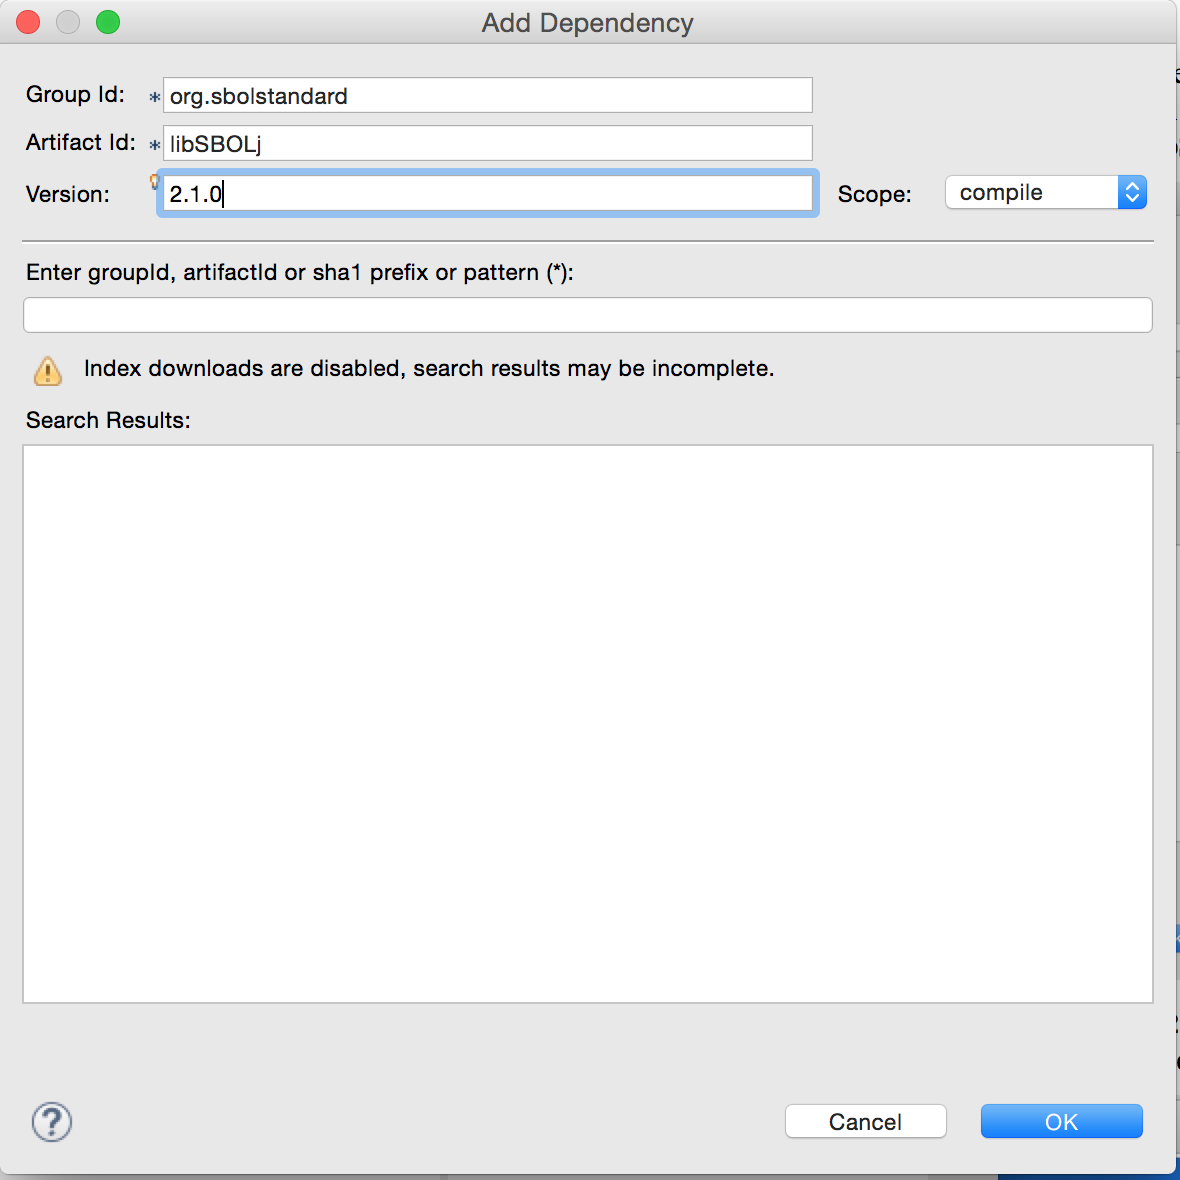
\includegraphics[width=0.55\textwidth]{figures/addMavenDependency2}
\end{center}

After this dependency is added, Maven automatically brings in the  {\tt libSBOLj-2.1.0.jar} and its dependencies from the Maven Central Repository, and places them under the {\bf Maven Dependencies} directory.
\begin{center}
  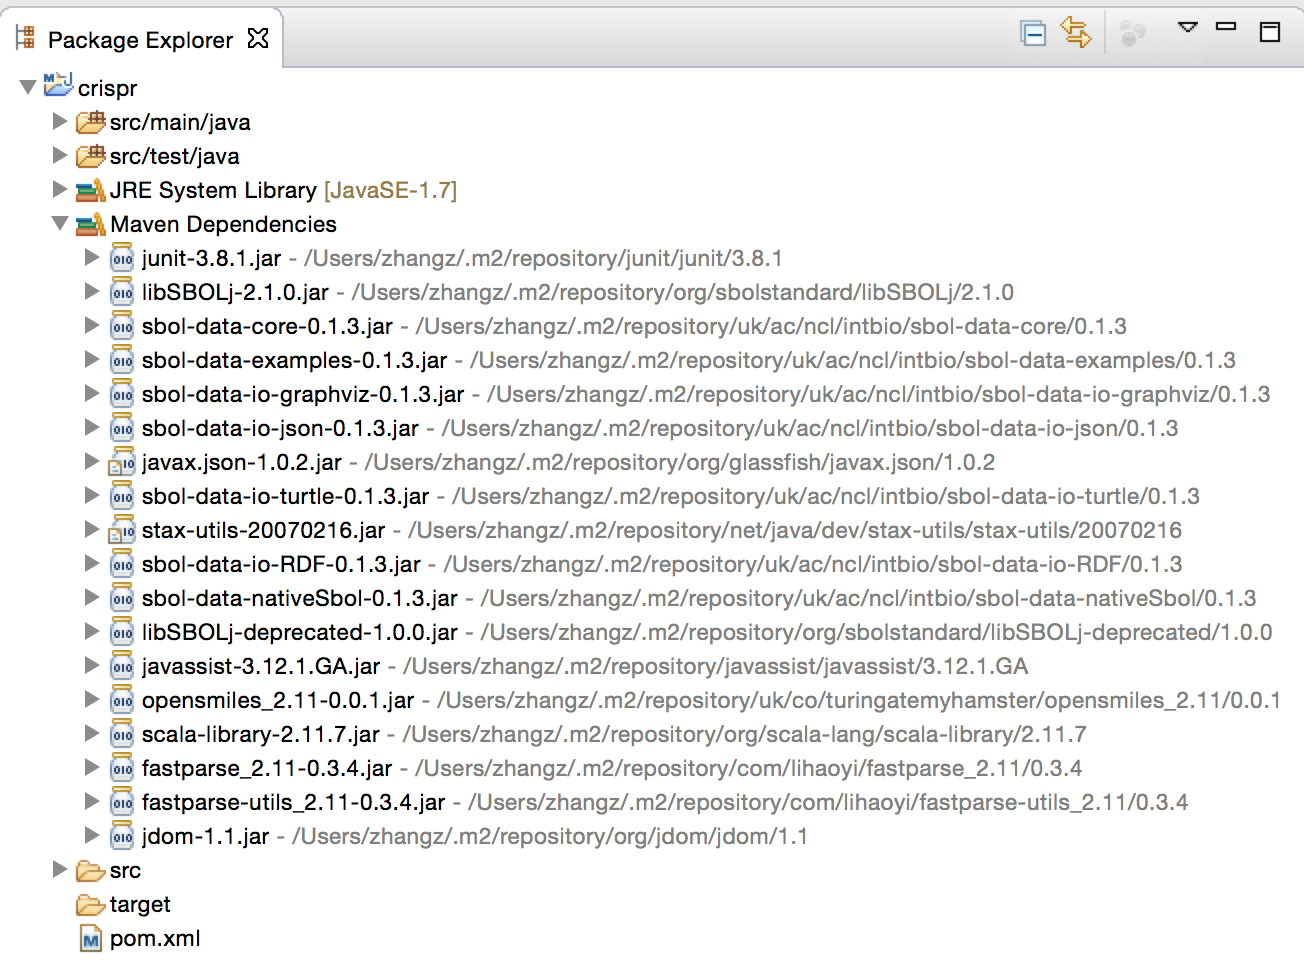
\includegraphics[width=0.8\textwidth]{figures/addMavenDependency3}
\end{center}


